% Chapter Template

\chapter{Resultados} % Main chapter title

\label{Chapter4} % Change X to a consecutive number; for referencing this chapter elsewhere, use \ref{ChapterX}

%----------------------------------------------------------------------------------------
%	SECTION 1
%----------------------------------------------------------------------------------------

\section{Resultados}
\label{sec: Resultados}

\subsection{Resultados de ensayos con marcos de prueba}

\subsubsection{FFD. Ensayo 1}

Se introdujo los siguientes estímulos:
\begin{itemize}
\item Señal de reloj de 1 ns de periodo.
\item Señal de video de entrada \texttt{d\_ffd\_tb} de \texttt{14\-bit} cuyo valor crece cada 1 ns.
\item Señal de habilitación \texttt{en\_ffd\_tb} con valor permante en '1' lógico (siempre habilitado).
\item Señal de reset \texttt{rst\_ffd\_tb} con valor permanente en '0' lógico (nunca resetea).
\end{itemize}

\begin{figure}
\centering
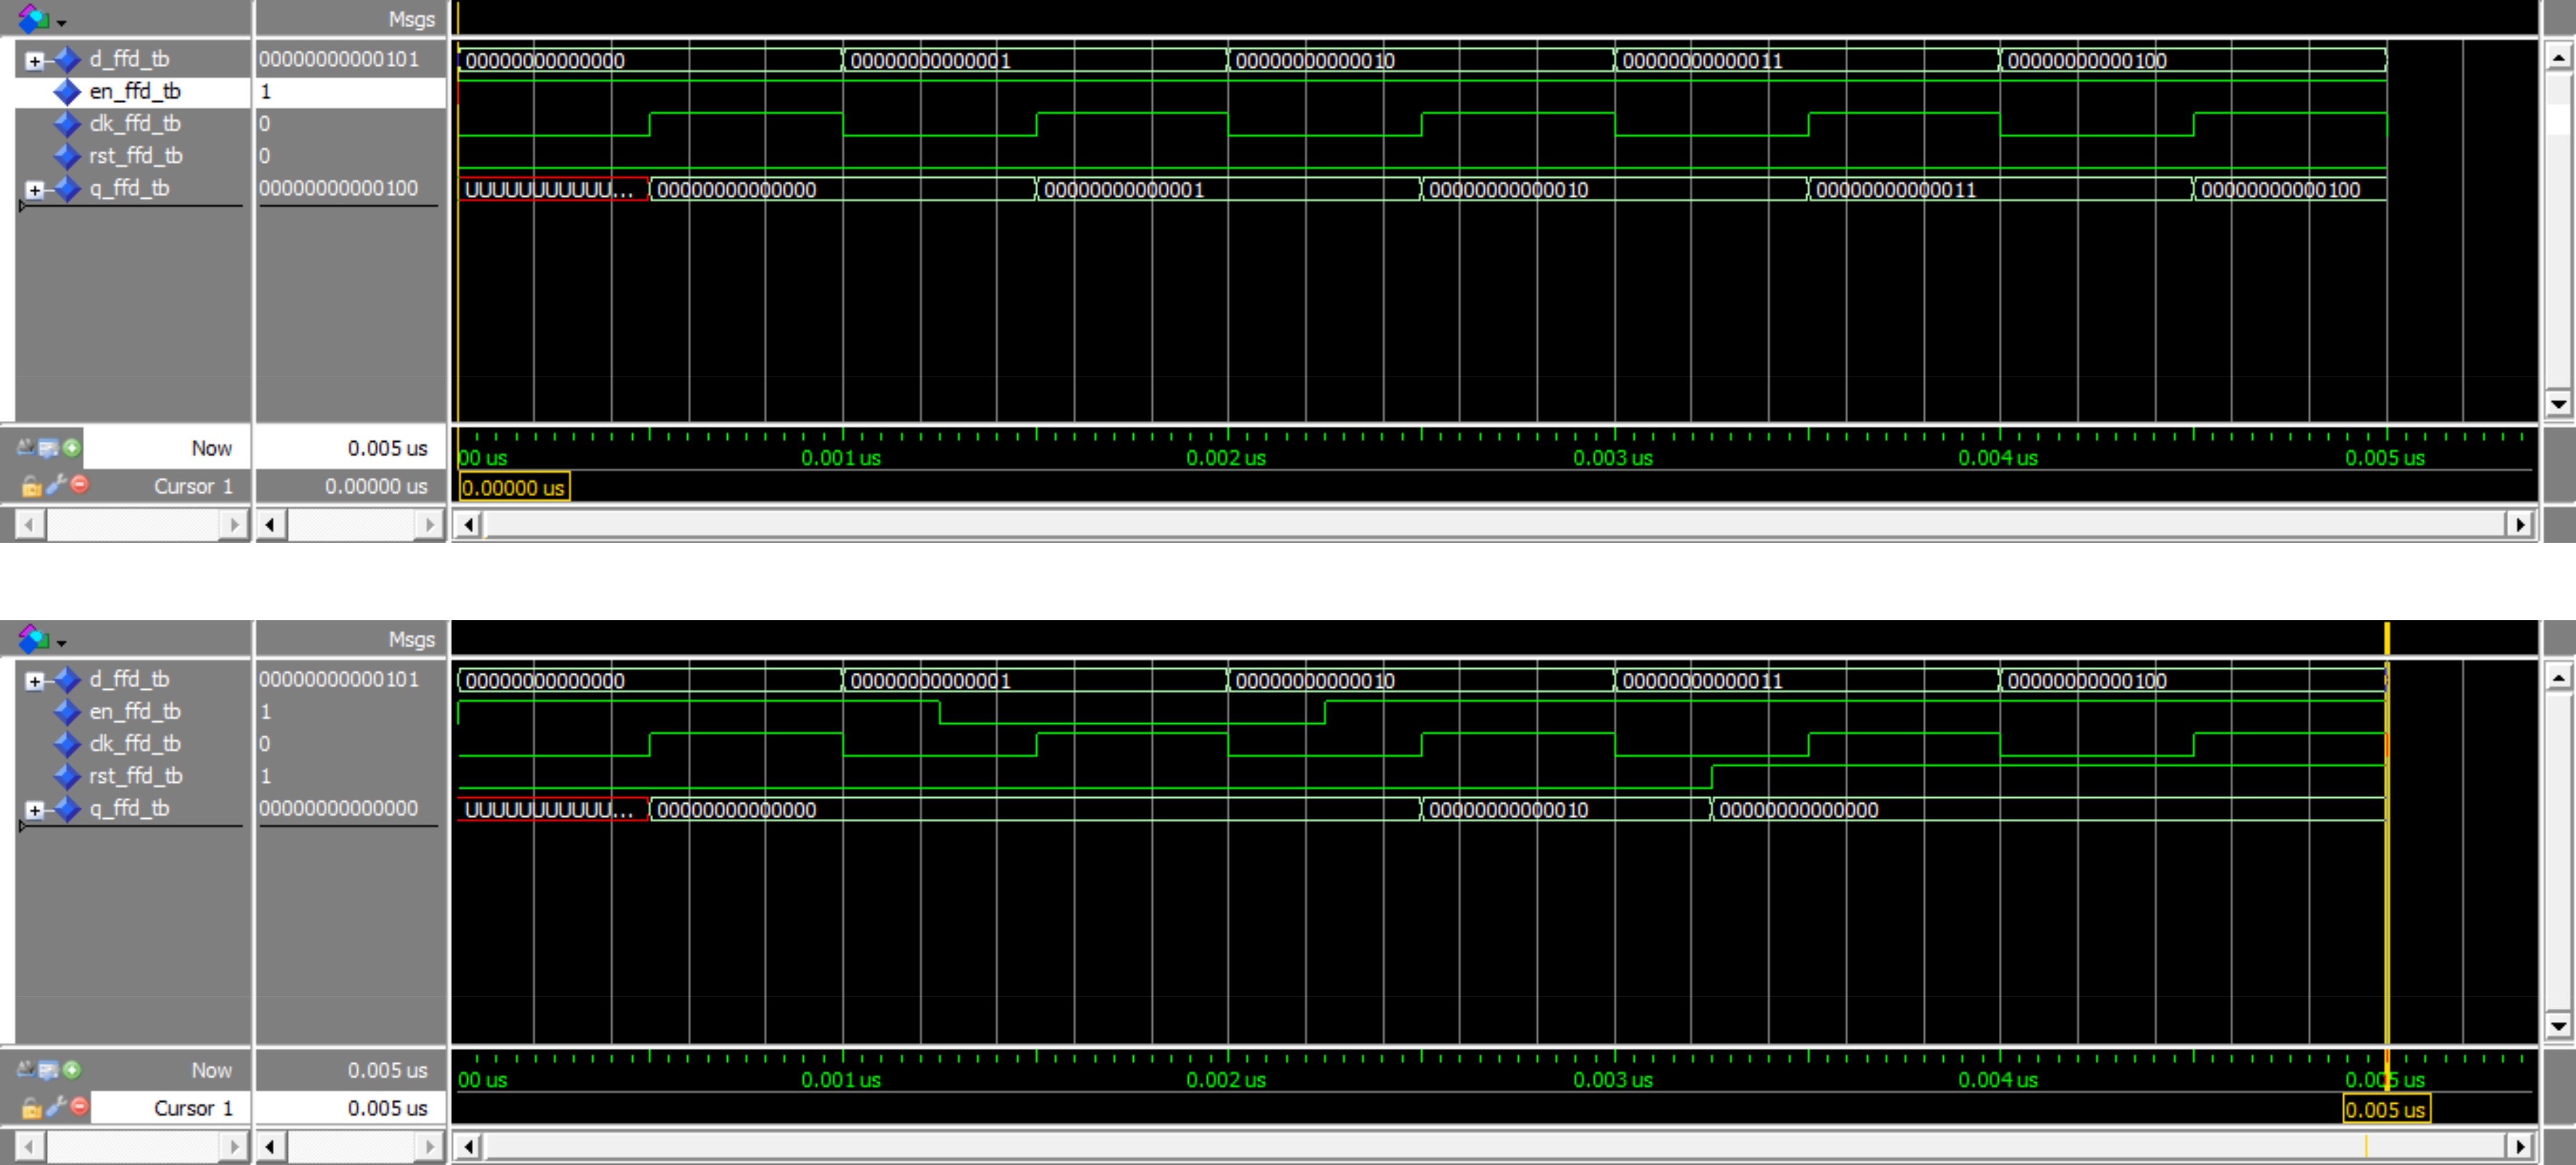
\includegraphics[scale=0.2, angle=270]{./Figures/tb_cfar_ffd.png}
\caption{Ensayo 1 (derecha) y 2 (izquierda) sobre el módulo "ffd"}
\label{tb_cfar_ffd}
\end{figure}

Los resultados se ilustran en la parte derecha de la figura \ref{tb_cfar_ffd}. Se observó en la señal de salida \texttt{q\_ffd\_tb} que:

\begin{itemize}
\item En los primeros 5 ns la salida está indefinida. Lo cual es esperable.
\item En cada flanco ascendente del reloj el valor de la señal de entrada se transfiere al puerto de salida.
\end{itemize}

Los comportamientos son esperados.


\subsubsection{FFD. Ensayo 2}

Se introdujo los siguientes estímulos:
\begin{itemize}
\item Señal de reloj de 1 ns de periodo.
\item Señal de video de entrada \texttt{d\_ffd\_tb} de 14-bit cuyo valor crece cada 1 ns.
\item Señal de habilitación \texttt{en\_ffd\_tb} con valor '1' lógico durante los primeros 1.25 ns, '0' lógico entre 1.25 y 2.25 ns, y '1' lógico luego de 2.25 ns.
\item Señal de reset \texttt{rst\_ffd\_tb} con valor '0' lógico hasta 3.25 ns y '1' lógico luego de 3.25 ns.
\end{itemize}


Los resultados se ilustran en la parte izquierda de la figura \ref{tb_cfar_ffd}. Se observó en la señal de salida \texttt{q\_ffd\_tb} que:

\begin{itemize}
\item En los primeros 5 ns la salida está indefinida. Lo cual es esperable.
\item En primer flanco ascendente del reloj (5 ns) el valor de la señal de entrada se transfiere al puerto de salida.
\item Entre 5 ns y 2.25 ns la salida se mantiene en el valor anterior ("00000000000000"). Es decir, en el segundo flanco ascendente del reloj el valor de la señal de entrada \textbf{no} se transfiere a la salida. En este mismo intervalo se observa un nivel bajo de la señal de habilitación, lo que significa que \textit{no} está habilitado la tranferencia del dato de la entrada a la salida y un nivel bajo de la señal de reset (reset inactivo).
\item En el tercer flanco ascendente del reloj (2.5 ns) ocurre la transferencia del dato de la entrada a la salida, correspondiente al nivel alto de la señal de habilitación y al nivel bajo de la señal de reset.
\item Desde 3.5 ns hasta el final de la simulación, lo que incluye el cuarto y quinto flanco ascendente del reloj, se observa que el dato de salida es "00000000000000". Esto se corresponde con el cambio de nivel bajo a nivel alto de la señal de reset. Esto provoca que la salida se resetee.
\end{itemize}

Los comportamientos son esperados.


\subsubsection{Celdas de guarda. Ensayo 1}

Se introdujo los siguientes estímulos:
\begin{itemize}
\item Señal de reloj de 1 ns de periodo.
\item Señal de video de entrada \texttt{d\_ffd\_tb} de 14-bit cuyo valor crece cada 1 ns.
\item Señal de habilitación \texttt{en\_ffd\_tb} con valor permante en '1' lógico (siempre habilitado).
\item Señal de reset \texttt{rst\_ffd\_tb} con valor permanente en '0' lógico (nunca resetea).
\end{itemize}

\begin{figure}
\centering
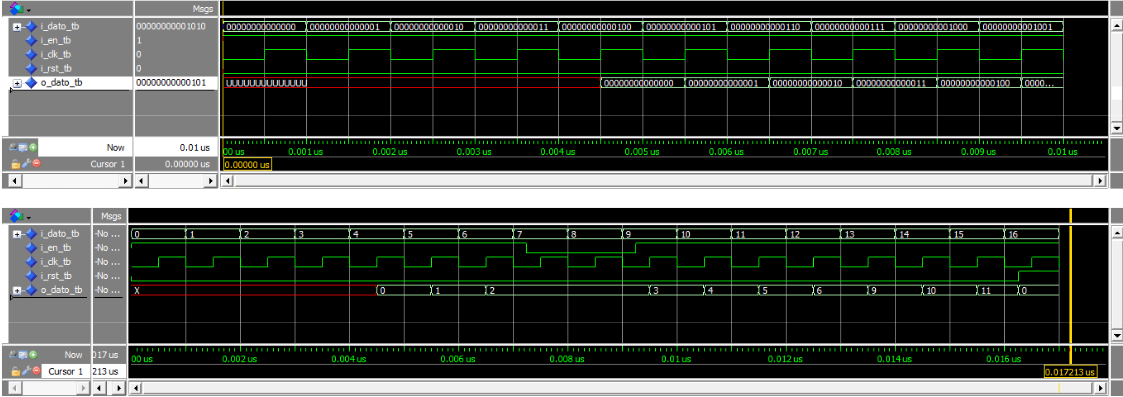
\includegraphics[scale=0.85, angle=270]{./Figures/tb_cfar_gc.png}
\caption{Ensayo 1 (izquierda) y 2 (derecha) sobre el módulo 'celdas de guarda'}
\label{tb_cfar_gc}
\end{figure}

Los resultados se ilustran en la parte izquierda de la figura \ref{tb_cfar_gc}. Se observó en la señal de salida \texttt{q\_ffd\_tb} que:

\begin{itemize}
\item En los primeros 5 ns la salida está indefinida. Lo cual es esperable.
\item En cada flanco ascendente del reloj el valor de la señal de entrada se transfiere al puerto de salida.
\end{itemize}

Los comportamientos son esperados.


\subsubsection{Celdas de guarda. Ensayo 2}

Se introdujo los siguientes estímulos:
\begin{itemize}
\item Señal de reloj de 1 ns de periodo.
\item Señal de video de entrada \texttt{d\_ffd\_tb} de 14-bit cuyo valor crece cada 1 ns.
\item Señal de habilitación \texttt{en\_ffd\_tb} con valor '1' lógico durante los primeros 1.25 ns, '0' lógico entre 1.25 y 2.25 ns, y '1' lógico luego de 2.25 ns.
\item Señal de reset \texttt{rst\_ffd\_tb} con valor '0' lógico hasta 3.25 ns y '1' lógico luego de 3.25 ns.
\end{itemize}


Los resultados se ilustran en la parte derecha de la figura \ref{tb_cfar_gc}. Se observó en la señal de salida \texttt{q\_ffd\_tb} que:

\begin{itemize}
\item En los primeros 5 ns la salida está indefinida. Lo cual es esperable.
\item En primer flanco ascendente del reloj (5 ns) el valor de la señal de entrada se transfiere al puerto de salida.
\item Entre 5 ns y 2.25 ns la salida se mantiene en el valor anterior ("00000000000000"). Es decir, en el segundo flanco ascendente del reloj el valor de la señal de entrada \textbf{no} se transfiere a la salida. En este mismo intervalo se observa un nivel bajo de la señal de habilitación, lo que significa que \textit{no} está habilitado la tranferencia del dato de la entrada a la salida y un nivel bajo de la señal de reset (reset inactivo).
\item En el tercer flanco ascendente del reloj (2.5 ns) ocurre la transferencia del dato de la entrada a la salida, correspondiente al nivel alto de la señal de habilitación y al nivel bajo de la señal de reset.
\item Desde 3.5 ns hasta el final de la simulación, lo que incluye el cuarto y quinto flanco ascendente del reloj, se observa que el dato de salida es "00000000000000". Esto se corresponde con el cambio de nivel bajo a nivel alto de la señal de reset. Esto provoca que la salida se resetee.
\end{itemize}

Los comportamientos son esperados.